% Chapter 1

\chapter{Introduction}

\label{chap:introduction} 

\graphicspath{{Figures/Introduction}}

Programming languages are the media through which we communicate our ideas with machines, be it mathematical formulae or video games. Like human languages, programming languages consist of words, grammar, and meaning. Unlike conversing with humans, machines tolerate very little ambiguity and are not skillful at navigating confusion. Therefore, sometimes inconsistencies glossed over by humans can cause unexpected results in computer programs; a missing semicolon or extra empty space can lead to entirely different outcomes, sometimes resulting in disastrous failures. Throughout the history of programming, various ways were invented to ensure the program behaves as expected. Through this, a pattern emerges from our pursuit for program correctness: the more certainty a programmer attains through programming language rules and checks that their program will run correctly, the more difficulty the programmer has in conforming to those rules and checks. Further, when these rules and checks are violated, we meet the anguish of the machine in arcane jargon, sometimes all in uppercase letters.

In this thesis, we investigate the problem of type errors, a common way for machines to signal that the program failed a safety check. Although they are intended to guide programmers in writing better code, type errors are known to instill fear in beginner programmers and remain a persistent annoyance for even experienced developers. We identify what causes type errors, why they are hard to deal with, and why our existing tools fall short to help programmers combat type errors. We introduce our interventions, most notably, \chameleon{} (Chapter \ref{chap:chameleon}), Goanna (Chapter~\ref{chap:goanna}), and GeckoGraph (Chapter~\ref{chap:gecko-graph}), aimed to transform the traditional, often terse, type error feedback into a dynamic and clear diagnostic system enhanced by interactive user interfaces. 


In this chapter, we delve into two critical aspects of programming language design: their typing disciplines (Section \ref{sec:typing}) and the paradigms to which they subscribe (Section \ref{sec:paradigm}). We discuss the nature of type errors, their characteristics (Section \ref{sec:symptoms}), and the inherent complexities associated with improving them (Section \ref{sec:challenges}). Furthermore, we review the evolution of tools designed to aid programmers in deciphering and resolving program errors (Section \ref{sec:debugging-tools}), addressing the notable gap between the tools to support type errors and runtime errors. Through these discussions, we seek to illuminate both the challenges and the ongoing efforts to enhance type error diagnostics.

% Through this, we hope to illustrate a common trade-off in programming: the more certainty a programmer attains through programming language rules and checks that their program will run correctly, the more difficulty the programmer has in conforming to those rules and checks. Further, when these rules and checks are violated, we meet the anguish of the machine in arcane jargon, sometimes all in uppercase letters.





% \begin{itemize}
%   \item \textbf{Clarity}: We aim to provide succinct and accurate explanations of errors, cutting through unfamiliar terminologies, awkwardly phrased sentences, and excessive amounts of unhelpful information that often obscure the underlying issues.
%   \item \textbf{Intuitiveness}: Our systems are designed with user-friendly interfaces that are easy to learn, comprehend, and use, ensuring that programmers of all skill levels can efficiently navigate and rectify errors.
%   \item \textbf{Confidence}: Building on solid foundations in programming language theory and constraint satisfiability research, our tools maintain the rigorous program safety features expected from traditional compilers, while enhancing the user experience.
% \end{itemize}

% Through these innovative systems, we strive to demystify error messages and equip programmers with better tools to write correct programs. 


\section{From types to program correctness}
\label{sec:typing}
In programming language theory and practice, type systems are a widely adopted program validation method where types of expressions are checked against their usage. In the early history of programming, types were used to inform the compiler of how much memory needed to be allocated for each value. Now, type systems are much more powerful; programmers can express complex ideas, like communication protocols and concurrency characteristics. Conventionally, the discipline of typing is identified by the existence of a compile-time checking stage. A programming language is said to be \textbf{statically typed} if checks are performed before a program is executed.  On the other hand, \textbf{dynamically typed} languages (colloquially called dynamic languages) will not complain about type mismatch prior to the program being run, and they do not facilitate describing the types (Fig.\ \ref{fig:typed-vs-untyped}). In dynamic languages, expressions like \texttt{4 + "2"} may produce unintended consequences, for example, a runtime error causing the program to terminate early, or some languages may try to perform unexpected coercion of data types, producing the answer ``42'' (i.e.\ string concatenation instead of numeric addition). 

Statically typed languages have a long history and are extremely popular, with examples among both the earliest of programming languages (such as FORTRAN \cite{Backus1978-xt} and ALGOL) and the most widely used languages across all platforms (such as C~\cite{Ritchie1978-pa}---and its derivatives, including Java and C\#). Static typing is also a core feature of the most advanced and renowned academic languages (such as ML and Haskell~\cite{Hudak2007-kn} --- as well as their derivatives, such as OCaML and Agda, respectively). In practice, statically typed programming languages offer many advantages. Type declarations and annotations add important contextual information about the expected use of variables and expressions. This additional context allows early error detection but also enhances code readability and promotes maintainability \cite{Kleinschmager2012-bg}, especially in large collaborative projects. Explicitly written type annotation also creates opportunities to improve tooling support through intelligent compiler services and IDE (interactive development environment). Additionally, static typing enhances code documentation by clarifying contracts between library authors and users and, more generally, enhancing code reusability \cite{Endrikat2014-uz}.


In comparison, dynamic typing has its own benefits and has an equal, if not stronger, influence in the computing world. In dynamically typed languages, a variable can hold different types of values because the type is checked during runtime. This often provides more flexibility than static typing since a function can be used to process different types of input values without any special semantics. However, this flexibility also carries risks, such as the example expression \texttt{4 + "2"}, where continuing execution with an incorrect value could have dire outcomes, especially when running in a production environment.
%: expressions like \texttt{4 + "2"} will not be identified before executing the program; some languages try to perform unexpected coercion of data types to avoid errors, producing the answer ``42''. 

Languages within the Lisp family, such as Common Lisp and Scheme, epitomize the advantages of dynamic typing. In these languages, a prevalent design pattern involves functions accepting potentially different Lisp data types: atoms, lists, or symbolic expressions (S-expressions). The function's behavior changes based on the runtime inspection of these inputs. Additionally, dynamic languages often have a lower learning curve. Programmers are not burdened with declaring and adhering to strict type constraints, allowing them to focus more on immediate computational tasks. In the modern computing landscape, the popularity of dynamic languages like JavaScript and Python can be attributed to their flexibility and ease of use, which significantly lowers the barrier to entry for new programmers \cite{Chatley2019-uq}.


It comes as no surprise that large amounts of work were dedicated to deciding which one of the two typing disciplines is superior. Over the years, numerous studies have attempted to compare these typing disciplines and their impact on various aspects of software development, including code quality \cite{Ray2017-gq, Gao2017-xn}, maintainability \cite{Kleinschmager2012-bg}, error resolution \cite{Prechelt1998-pd}, development speed for new features \cite{Prechelt2000-bf, Mayer2012-ko}, and comprehensibility \cite{Endrikat2014-uz}. Unfortunately, these studies have not led to a consensus, as the impacts of the typing disciplines can often be overshadowed by more dominating factors such as the style of the programming languages used and the skill levels of the programmers involved.

Despite the lack of universal agreement, conventional wisdom suggests that dynamically typed languages are often more suited for beginners and rapid prototyping, thanks to their flexibility and ease of use. Conversely, statically typed languages are typically favored in larger projects or environments where ongoing feature development and team collaboration are prevalent. This preference is due to the inherent type safety features, which help manage complexity and reduce certain errors as projects scale \cite{Chatley2019-uq}.


\begin{figure}[ht]
  \centering
  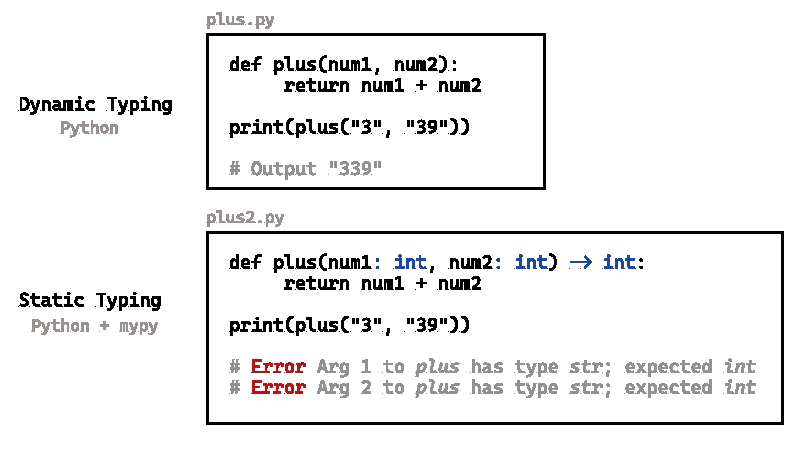
\includegraphics[width=\linewidth]{TypedVsUntyped.pdf}
  \caption[Comparison of the same program dynamically typed in Python and with mypy—a static typing tool for Python]{
    \label{fig:typed-vs-untyped}
    Comparison of the same program dynamically typed in Python (Top) and with mypy—a static typing tool for Python (Bottom).  The dynamic-typing rules of the Python interpreter apply, at run-time, the string concatenating version of the `+' operator -- regardless of the programmer's intention.  By contrast, mypy static-typing checks the type of the values passed to the {\tt plus} function against the intention declared by the programmer through the type annotations on the function parameters (both {\tt int}) and its return type (also {\tt int}).  The type check will fail until the programmer amends the function call with numeric arguments or otherwise explicitly converts the values from {\tt str} to {\tt int}.
    }
\end{figure}



\section{Functional Programming}
\label{sec:paradigm}
Alongside static typing, \textbf{functional programming} represents another rigorous approach to software development, drawing inspiration from Alonzo Church's lambda calculus in the 1930s \cite{Church1985-bx}. In functional programming languages, functions are the fundamental building blocks. They can be used as ordinary values, serving as both inputs and outputs for other functions, and can be combined to construct new functions. Programming in these languages centers around the composition of functions to perform high-level tasks. 
% Pure functional programming languages, characterized by immutable values and referential transparency, promote mathematical rigor. Immutable values ensure that once a value is declared, it cannot be altered. Referential transparency guarantees that functions will always produce the same output for identical inputs, providing predictable and testable code.

 A specific subset of functional programming languages, known as `pure' functional programming languages, incorporates additional mathematical rigor through concepts such as immutable values and referential transparency. Immutable values mean all values, once declared, cannot be modified. Referential transparency ensures that functions do not perform tasks that depend on external systems, such as reading from a global state, connecting to network resources, or even printing to the console.  These properties help mitigate undesirable programming behaviors similar to the way static typing does. For example, functional programming avoids issues like misaligned pointers and race conditions by disallowing mutable pointers and shared memory. Consequently, programs developed using these languages are more predictable and can be robustly tested and reasoned about \cite{Hu2015-ch}. This significantly reduces the risks that external factors could unpredictably affect program behavior, such as network fluctuations or even the passing of time \cite{Suzuki2019-bi}.

Functional programming is often advocated as an excellent choice for introductory programming courses due to its emphasis on mathematical reasoning and strict programming discipline \cite{Joosten1993-be, Chakravarty2004-ux}. This discipline includes the clear separation of data from its transformations, fostering a structured approach to problem-solving.


\begin{figure}[htbp]
  \centering
  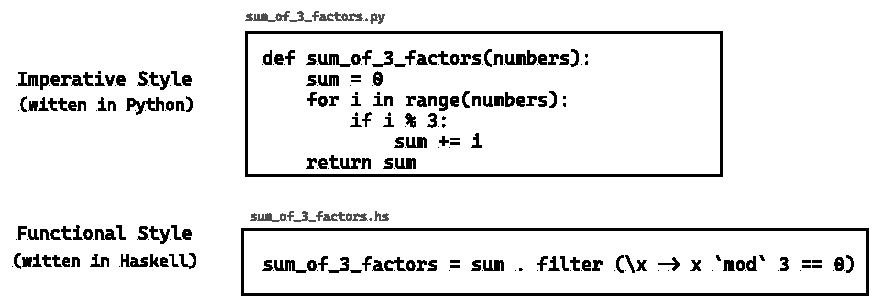
\includegraphics[width=\linewidth]{ImperativeFunctional}
  \caption[Comparing two approaches to implementing the same function specification in different programming paradigms: imperative and functional]{
    \label{fig:imperative-vs-functional}
    The figure compares two approaches to implementing the same function specification in different programming paradigms: imperative (top) and functional (bottom). The top section presents Python code, utilizing a loop and a mutable variable to accumulate sums. Conversely, the bottom section illustrates Haskell code, using a composition of two functions: \texttt{sum} and \texttt{filter}, the latter using a specified predicate in the form of an anonymous function. This exemplifies how imperative programming relies on the mutable state (the \texttt{sum} variable) to track progress, whereas functional programming leverages high-level abstractions and recursion to achieve similar outcomes.    
    }
\end{figure}


Functional programming contrasts with other mainstream paradigms like object-oriented programming, which structures programs around objects combining data and behavior, and procedural programming, which focuses on a sequence of procedural steps. Despite the strengths of functional programming, object-oriented and procedural paradigms, exemplified by Java and C, respectively, remain more prevalent in commercial environments \cite{StackOverflow2023-cp, Cass2023-fa}. These paradigms benefit from extensive legacy codebases, broad third-party library support, robust tooling, and familiarity. Lastly, the rigor in functional programming languages may raise the barrier to entry for beginners. For example, in many pure functional languages, printing to the terminal window, generally considered a basic technique to observe the execution of the program, exposes programmers to profound concepts like monad and side effects, which can be daunting to those who are new to the language.  


\section{Statically Typed Functional Languages, The Best Of Both Worlds}
Combining the disciplines described above, \textbf{statically-typed functional languages} employ both static typing and the principles of functional programming. The most common statically typed functional languages include Haskell,  ML (with the OCaml dialect being the most popular among the family of ML languages), and F\#. 
Of these, Haskell is the only ``pure'' functional language, with all variables being immutable by default.
Descendents of Haskell, like Idris and Agda, include more advanced type-level features like dependent type and session type, allowing programmers to express extremely granular checks of potential software behavior before running the program. These languages often provide the strongest level of programming safety. It is often advertised that programs in these languages will be error-free if the source code passes the compiling stage, indicating that compilers are able to weed out a large number of programming errors. These safety properties allow statically typed functional languages to be used as proof assistants or formal verification tools. They prove the correctness (or incorrectness) of many systems, from web public key infrastructure \cite{Bhargavan2021-no} to microcontrollers used in space programs \cite{Mokhov2019-zj}. 

Despite these safety benefits, these languages' presence in the mainstream programming world remains underwhelming. This modest popularity is often attributed to high entry barriers, unfamiliarity with the paradigms, and advanced type systems that can be overwhelming for newcomers.

\section{Symptoms of Type Errors}
\label{sec:symptoms}
 The compiler is the medium through which programmers transform human intention into machine instructions. When encountering errors, compilers often act like Oracles in ancient history, revealing to programmers obscure messages that can lead to confusion and the wrong course of action. Many studies have investigated the ineffectiveness of compiler error messages \cite{Barik2017-gy, Becker2019-cs, Becker2016-kc}.  Our exploration is centered around type error messages (a subclass of compiler error messages) in the Haskell programming language and its leading compiler, Glasgow Haskell Compiler (GHC). It is vital to mention that the challenges discussed here concerning error messages are common across compilers for various statically typed languages. Below, we delve into specific issues often observed in type error messages.


 \subsection{Bias in Type Errors} 
 \label{subsec:bias}
 
A significant issue in type error messages is their inherent bias. Often, type errors can arise from multiple causes, but the error message might only highlight one. This issue is known as left-to-right bias in traditional type-checking algorithms—a notable shortcoming that limits the usability of error messages \cite{McAdam2002-vb, Lee1998-fx, Chen2014-ev}.  For instance, as shown in Figure \ref{fig:type-error-example}, a programmer likely intended to add two numbers using the \texttt{+} operator instead of mistakenly using the concatenation operator \texttt{++}. However, the type error reported by the compiler mistakenly points to the application of the integer literal \texttt{3}, failing to suggest the more probable cause. We explore left-to-right bias further in Chapter \ref{chap:haskell-type-checking}.

 \begin{figure}[htbp]
  \centering
  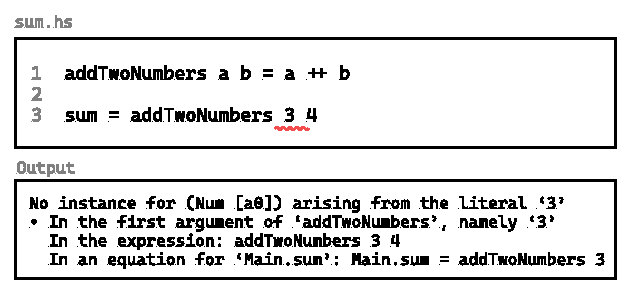
\includegraphics[width=\linewidth]{TypeErrorExample}
  \caption[Illustrating a programming error in Haskell, featuring a function named \texttt{addTwoNumbers} with a type error and the corresponding compiler output]{
    \label{fig:type-error-example}
    The figure illustrates a programming error scenario featuring the source code with a type error (Top) and the corresponding compiler output (Bottom). The error likely arises from the inappropriate use of the concatenation operator \texttt{++}, rather than the addition operator \texttt{+}, on line 1, as inferred from the function name \texttt{addTwoNumbers}. Despite this, the compiler erroneously highlights line 3, where the function \texttt{addTwoNumbers} is applied to the integer \texttt{3}, boldly assuming the correctness of the \texttt{addTwoNumbers} definition. This misdirection suggests a less likely source of error, potentially complicating the debugging process.
    }
\end{figure}


\subsection{Type Error Suggests Incomplete Cause}
\label{subsec:imcomplete}

Often, type error messages do not fully present all the locations relevant to the type error. Addressing the error at the recommended location might not suffice to resolve the underlying problem. Consider the scenario in Figure \ref{fig:type-error-example-2}, where a function intended for list concatenation is erroneously applied to integer values. Here, the error message only reports the first argument \texttt{3}, neglecting the second. This partial reporting leads to a situation where correcting the first argument to a list format, say \texttt{[3]}, doesn't rectify the error entirely; rather, it only updates to a slightly different error message. 



\begin{figure}[htbp]
    \centering
    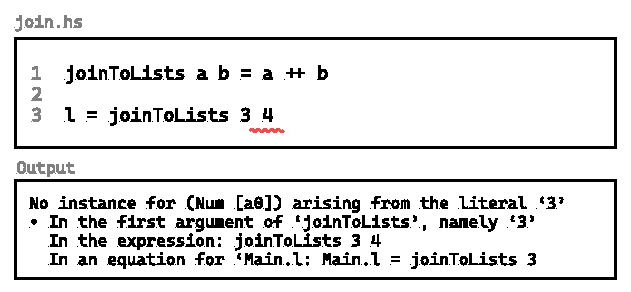
\includegraphics[width=\linewidth]{TypeErrorExample2}
  \caption[Illustrating a programming error in Haskell, featuring a function named \texttt{joinTwoLists} with a type error and the corresponding compiler output]{
    \label{fig:type-error-example-2}
    This figure depicts the same program as in Figure \ref{fig:type-error-example}, with one modification being the renaming of the function from \texttt{addTwoNumbers} to \texttt{joinTwoLists}. This change shifts the implied intent towards concatenating two \texttt{List} type values. The compiler still identifies an error at the same location—the integer literal \texttt{3}—aligning more closely with the programmer's understanding than in the previous example. However, the error message still misleadingly overlooks the erroneous type of the second argument, \texttt{4}, as it, too, is an invalid input for a list concatenation operation. Therefore, modifying only the first argument is insufficient to correct the type error.
    }
\end{figure}

\subsection{Missing Links In Type Errors}
\label{subsec:missing-link}

One of the most frustrating aspects of type errors is that they do not show the complete pathway of how the compiler decided on the type error. In the example in Fig \ref{fig:type-error-example-3}, the programmer may intend to compare to a char literal \texttt{' '} instead of string literal \texttt{" "} on line 1 in the function \texttt{isSpace}. However, multiple clues contribute to this conclusion. The definition of the function \texttt{trimWhiteSpace}, the application of \texttt{filter isSpace a}, the definition of \texttt{isSpace}, and even the type signature of \texttt{filter} all contribute to the logical reasoning. However, none of these are included in the actual error message.


\begin{figure}[htbp]
\centering  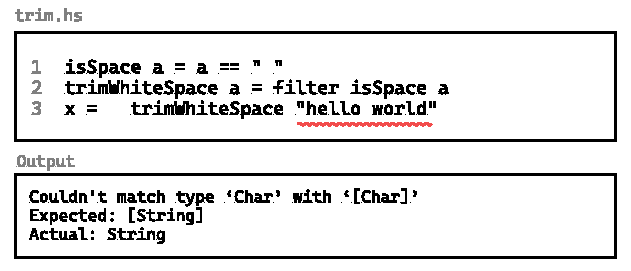
\includegraphics[width=\linewidth]{TypeErrorExample3}
  \caption[A type error in Haskell involving a type mismatch across multiple functions]{
    \label{fig:type-error-example-3}
    In Haskell, the \texttt{String} type is an alias for \texttt{[Char]}, meaning the two types are equivalent. The function \texttt{trimWhiteSpace}, as used on line 3, processes a \texttt{String} (or list of \texttt{Char} values) to filter out whitespace characters. However, the function’s filter condition, \texttt{isSpace}, erroneously compares two \texttt{String} values instead of \texttt{Char} types. This is likely a type intending the char literal \texttt{' '} rather than the string literal \texttt{" "}. While the type error message correctly identifies the mismatch, it fails to provide crucial contextual clues that would obscure the nature of this error.
    }
\end{figure}


\subsection{The Use of Obscure Language}

Error messages are frequently plagued by technical jargon and convoluted phrasing, which can be particularly off-putting for novices. An example is the error message, \texttt{No instance for (Num a) arising from the literal `3'}, which is an inept way of suggesting a type mismatch involving character and numeric types. In fact, this is often the common behavior across many programming languages and has been shown in many studies \cite{Barik2017-gy, Tirronen2015-nr, Prather2017-dg}. Thus, concerted efforts \cite{Becker2016-kc, Barik2014-ib}  show that rephrasing the error message to be clearer and more structured positively affects programmers' ability to solve these errors.


\section{The Challenges Of Making Good Type Errors}
\label{sec:challenges}
After introducing some typical symptoms of bad type error messages, we now explore some fundamental challenges to improve type error messages.

\subsection{Types Are Complex}

The advantages of statically typed languages derive from their robust type-checking systems, which, ironically, also introduce significant complexities. Language and tool designers frequently overlook the intrinsic complexity of type systems.  Type checking in these languages can exhibit Turing-complete characteristics, which might lead to non-terminating processes~\cite{Wells1999-ob}. TypeScript introduces `conditional types', a feature that allows sophisticated computations at the type level (Fig. \ref{fig:ts-conditional}), posing challenges in explaining errors when these type-level computations fail due to a lack of adequate debugging tools.



\begin{figure}[htbp]
  \centering
  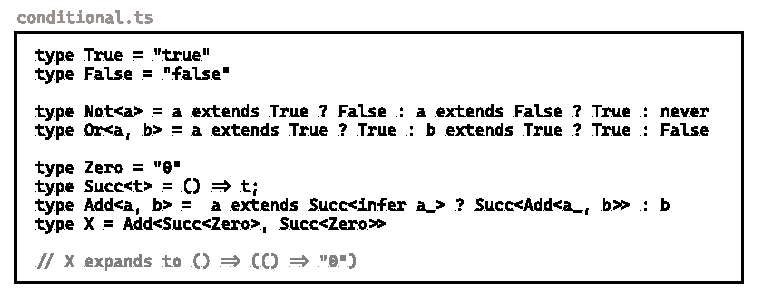
\includegraphics[width=\linewidth]{Conditional}
  \caption[An example of encoding propositional logic operators and church numerals in  TypeScript's conditional types]{
    \label{fig:ts-conditional}
    TypeScript includes a type-level feature known as `conditional types,' which enables the declaring of a type based on the outcome of a condition check. This capability is sufficient to construct a Turing-complete language within the TypeScript type system. The figure illustrates a simple language that supports booleans, numbers (using Church encoding), and functions that operate on these values. Since this implementation is implemented entirely at the type level, it does not generate any executable code for runtime evaluation, functioning purely within the compile-time environment. The recreational value aside, these type-level features often lead to elaborated ``essay of types'', hindering understanding and usability.
    }
\end{figure}

\subsection{Clues For Type Checking May Be Implicit}

The task of understanding how types are assigned in a program grows notably more complex when the programming language employs type inference. Type inference \cite{Damas1982-zw} is a technique that allows programmers to forgo the task of writing type annotations. Instead, the type checker automatically deduces the appropriate types for each expression based on the context. Although it succeeded in providing rigorous type checking without the hassle of manually writing type annotations, type inference has been shown to bring many usability issues \cite{Jun2002-xp, Wand1986-lu} for its implicitness.  

Even in programming languages that do not utilize implicit typing, certain typing rules remain opaque to programmers. For instance, rules on permissible values for equality check using the \texttt{==} operator vary across programming languages; some languages disallow comparison of lists, and others are fine with lists but disallow comparison of floating-point numbers. In languages that support a record data type, programmers must navigate additional complexities, such as whether adding or removing a field from a record maintains type correctness (Fig. \ref{fig:row-polymophism}). This often involves an understanding of nuanced language-specific rules, including concepts like covariance, contravariance, and subsumption.

\begin{figure}[htbp]
  \centering
  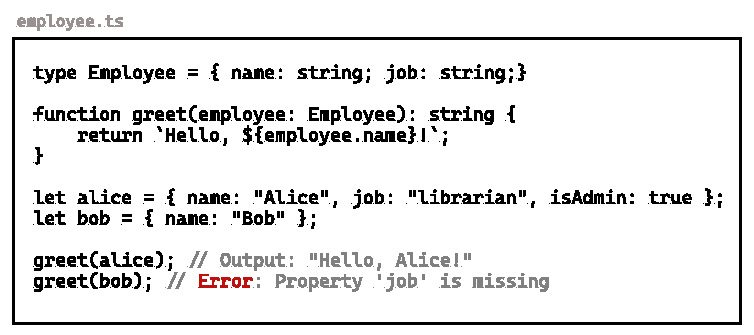
\includegraphics[width=\linewidth]{RowPolymorphism.pdf}
  \caption[An example of a correct usage and a wrong usage of row polymorphism in TypeScript]{
    \label{fig:row-polymophism}
Row polymorphism is a common type-level feature, allowing record values with optional more fields to be a subtype of the record without these fields. This enhances flexibility in structuring data collections but also introduces complexity in understanding the relations between types. The figure illustrates an example where programmers try to apply the record values \texttt{alice} and \texttt{bob} to the function \texttt{greet}. Because of the rules of row polymorphism and the fact that function arguments are covariant, only one value constitutes a valid input. 
    }
\end{figure}

These challenges amplify the difficulty in designing intuitive type error messages. The complexity of type systems demands that designers have a profound understanding of both theoretical and practical aspects of language implementation—knowledge often possessed only by the core language developers. Moreover, the implicit nature of modern programming languages requires that type errors be designed on a case-by-case basis, a daunting task given the limited number of contributors who possess the necessary expertise.

\section{The Lack of Type Debugging Tools}
\label{sec:debugging-tools}
Debugging programming errors have been an unpleasant but crucial part of programming since the inception of computing, tracing back to as early as 1949 \cite{Campbell-Kelly1992-rn}. However, the tools and support for debugging type errors have not evolved significantly and do not match the advancement of those available for runtime errors.

For runtime errors, one of the simplest and most effective debugging techniques is to insert \texttt{print} statements. As Brian W. Kernighan, one of the creators of the Unix system, once noted, ``The most effective debugging tool is careful thought, coupled with judiciously placed print statements'' \cite{Kernighan1978-xs}. Furthermore, breakpoint debugging has become a staple in nearly all programming Integrated Development Environments (IDEs), allowing for intermittent code execution and inspection (Fig. \ref{fig:breakpoint}). Research in error debugging tools continues to propose novel ideas. For instance, ZStep94 \cite{Lieberman1995-lg} enhances traditional breakpoint debugging by eliminating the need to set breakpoints, thus enabling programmers to view and navigate through the historical values that expressions take throughout execution (Figure \ref{fig:zstep94}). Another innovative tool, WhyLine \cite{Ko2009-uf}, aligns with the principles of a natural programming environment \cite{Myers2004-fy} by allowing programmers to ask ``why'' questions and ``why not'' questions about certain program behavior.

Despite these advancements in runtime debugging tools, the development of type debugging seems to have stagnated. Most programming languages and development environments still handle type errors in ways reminiscent of early languages like FORTRAN and ALGOL. In recent years, some modern programming languages like Elm and Rust have made efforts to improve type error reporting, but these enhancements are often superficial and do not fundamentally change the debugging experience \cite{Ferdowsi2023-au}.


\begin{figure}[ht]
  \centering
  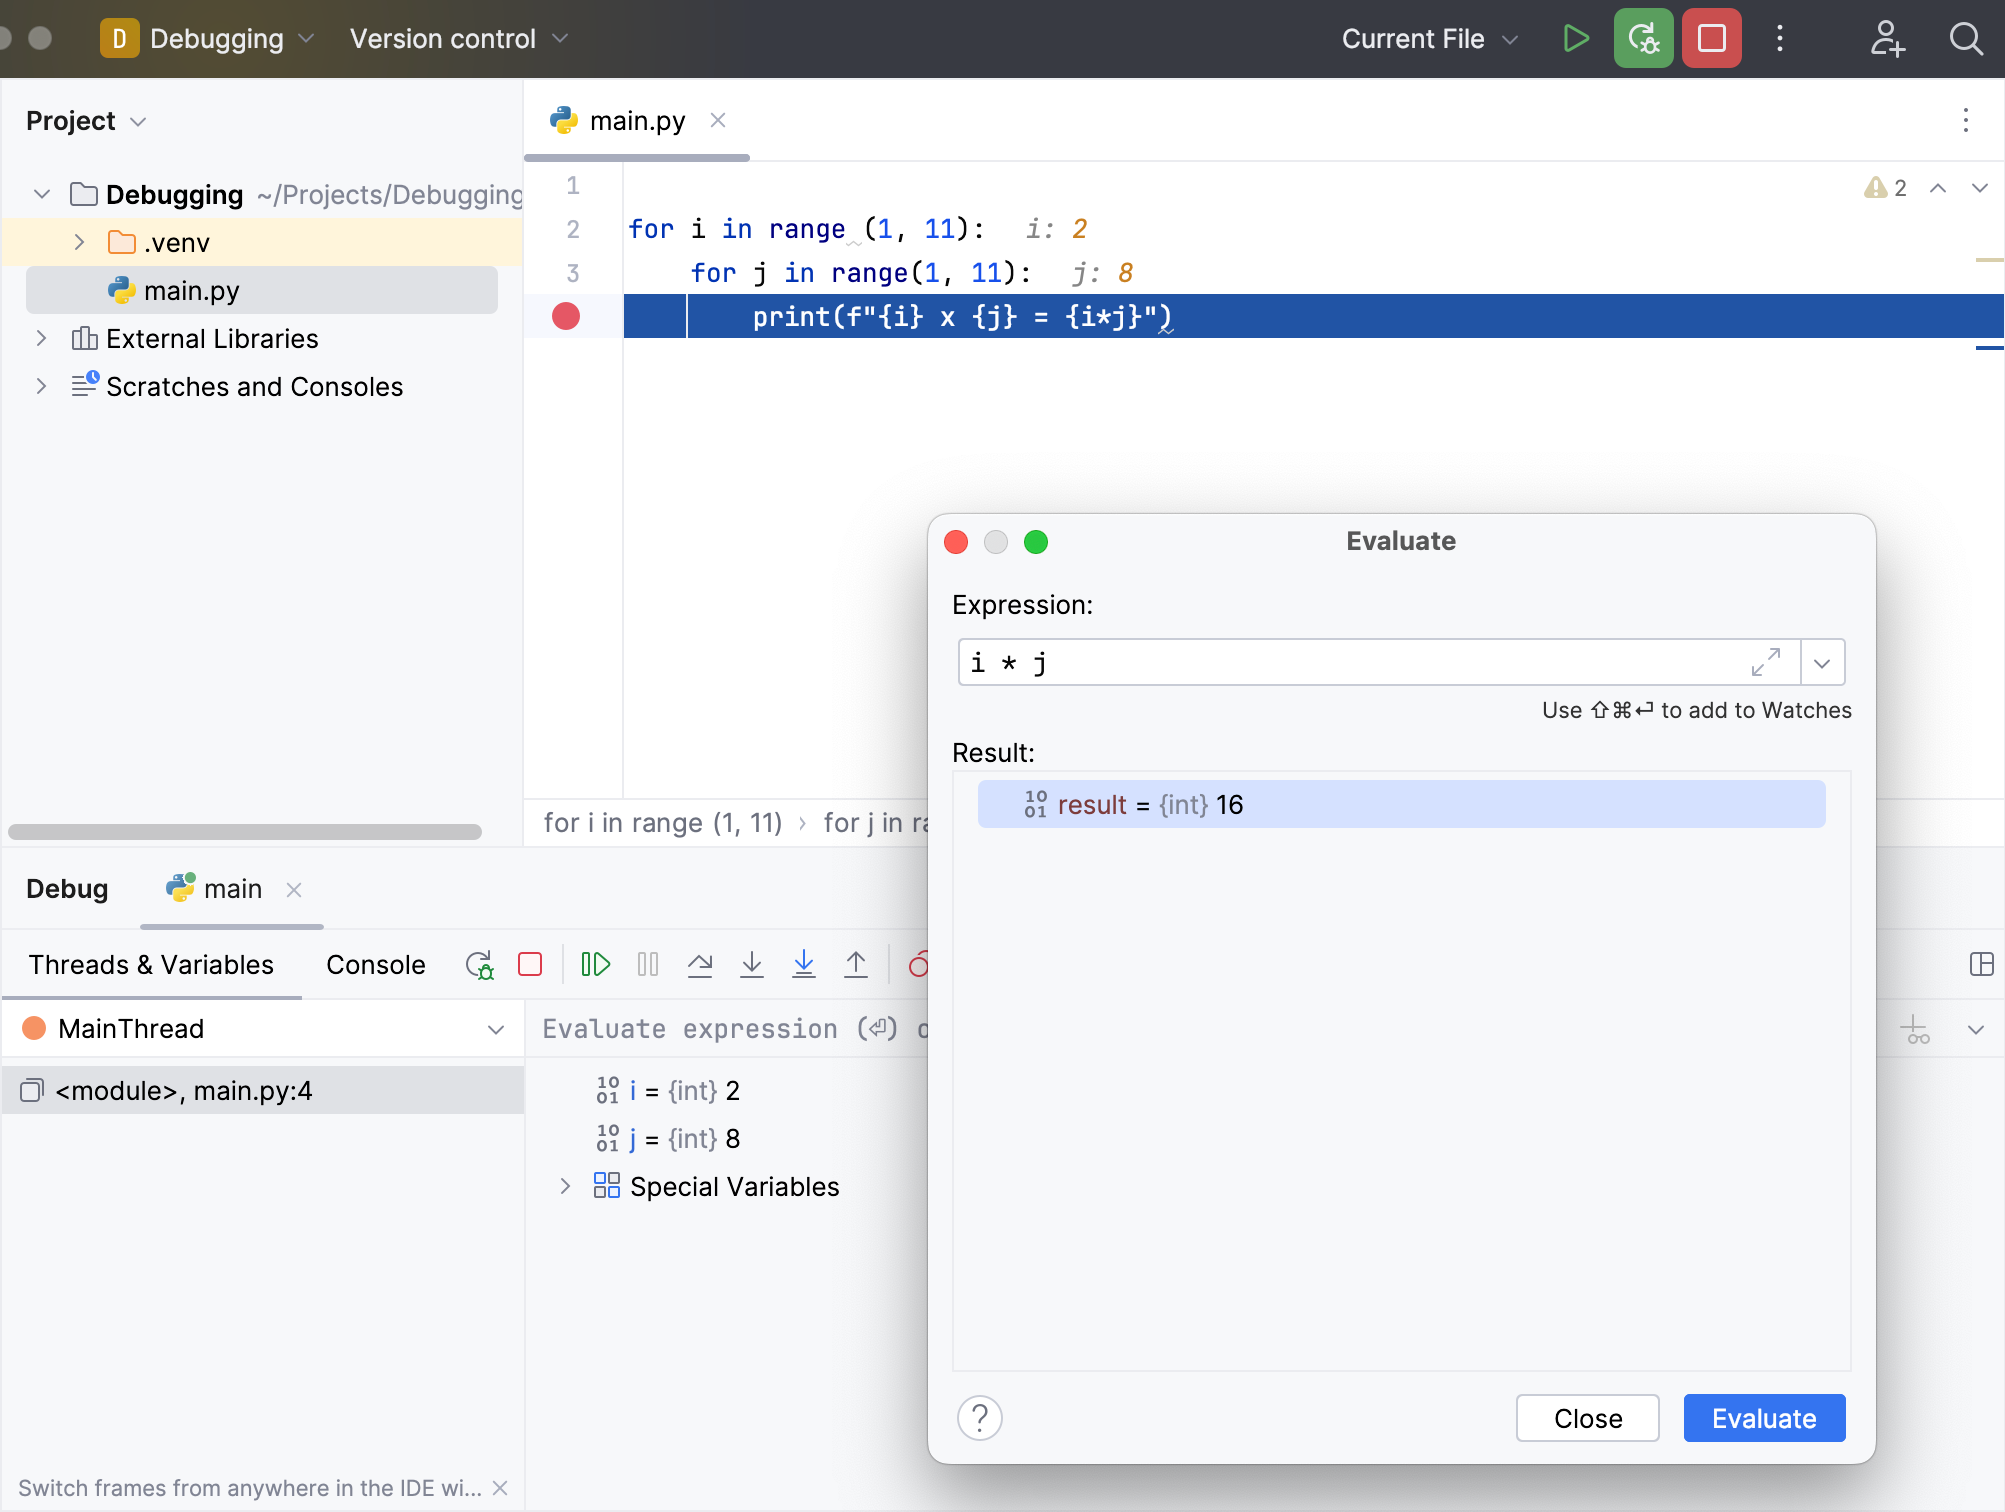
\includegraphics[width=\linewidth]{BreakPoint}
  \caption[Debugging of a Python program using a breakpoint and expression evaluation in PyCharm]{
    \label{fig:breakpoint}
    The figure shows the debugging of a Python program using a breakpoint and expression evaluation in PyCharm, a widely used interactive programming environment (IDE) for Python. Program execution is paused at the breakpoint set on line 4, and with each pause, the user-defined expression \texttt{i * j} is re-evaluated. This common debugging interface is available in nearly all modern programming editors and integrated development environments.
    }
\end{figure}


\begin{figure}[ht]
  \centering
  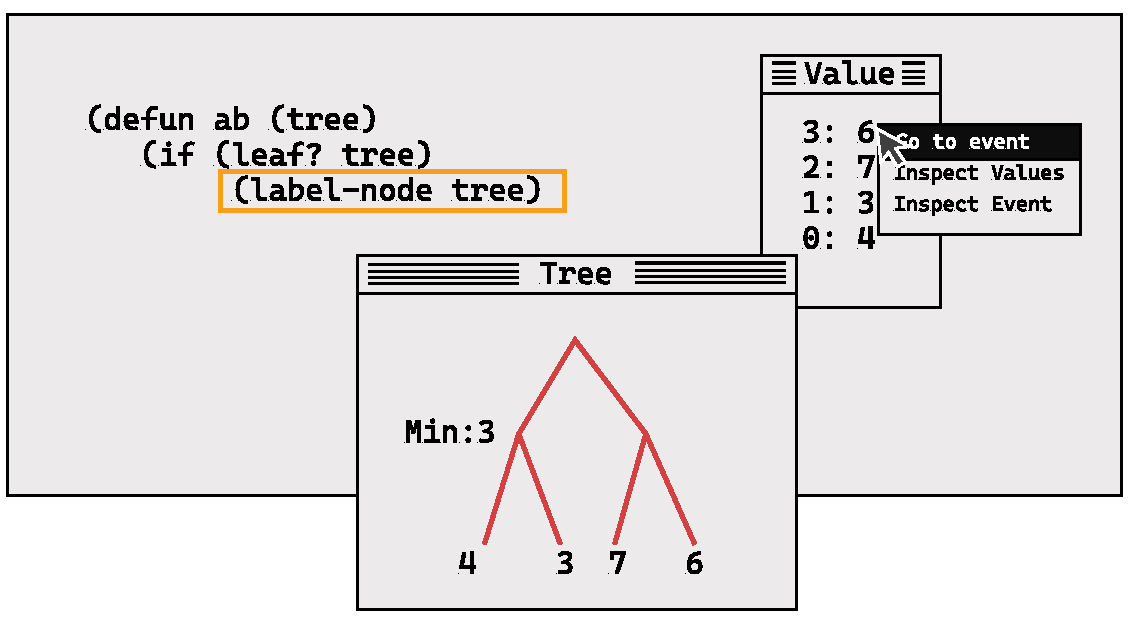
\includegraphics[width=\linewidth]{ZStep94}
  \caption[Debugging a Lisp program by inspecting all the historical values of an expression in ZStep94]{
    \label{fig:zstep94}
    Debugging a Lisp program by inspecting all the historical values of an expression, navigating through execution history, and reviewing live visualization replay.  All these features are provided in ZStep94.
    }
\end{figure}



\section{Research aim and objectives}

This research is driven by the acknowledged difficulties in debugging type errors and the lack of significant advancement in the tools and techniques used for presenting and resolving these errors. \textbf{We aim to improve both the usability and accessibility of type error diagnostics, making statically typed languages more approachable for developers at all levels of expertise}. To achieve this, we have established two main objectives in order to tackle the inherent complexity of type errors and provide the support tools to manage them.

\subsection{Objective 1. Provide programmers with the comprehensive knowledge needed to understand and resolve type errors.}
\label{subsec:aim1}

Current representations of type errors in most compiler tools are often insufficient for straightforward resolution without further investigation by the programmer. They typically provide only the location of the type check failure, the expected type, and the actual type encountered. This conventional approach, as discussed in the previous sections (\ref{sec:symptoms}), lacks practicality and clarity. We intend to address the need for a richer, more informative explanation of type errors by evaluating the limitations of existing systems and analyzing how programmers tackle type errors in practice.

\subsubsection{Objective 1.1 To Encompass Multiple Potential Causes Of A Type Error}
An essential aspect of this research is to challenge and expand beyond the bias found in traditional type error reporting (Section \ref{subsec:bias}). It is crucial to inform programmers that multiple potential causes and resolutions are almost certain to be present in every type error. A key goal is to communicate the dimension of multiple potential causes effectively. In addition, for each potential cause, programmers need a clear explanation of where the offending code is, which typing rules are violated, and, most importantly, how the meaning of the program will change after the error is resolved.


\subsubsection{Objective 1.2 To Accurately Report Relevant Locations Contributing to Type Errors.}
Current tools often pinpoint a single location for a type error, a method that has attracted considerable criticism for its inefficiency. Programmers frequently need to scan beyond the initially reported location. We propose to enhance type error reporting by identifying and detailing all relevant error-contributing locations across the codebase.

\subsubsection{Objective 1.3 To Give Reasons And Support Human Understanding}
Understanding type errors goes beyond pinpointing the location in the code. Internally, type errors can be caused by mismatched types, unmatched type class constraints, and trying to construct infinite types, among other reasons. Externally, type errors can be caused by typos, outdated type annotation, incomplete implementation, etc. Our goal is not only to locate these errors but to explain them in a way that logically supports the programmer's understanding and troubleshooting process, covering both internal causes and external causes.



\subsection{Objective 2. Support Programmers To Type Errors Through Interactive Modern Programming Environments.}

We focus on integrating comprehensive type error encoding (Section \ref{subsec:aim1}) within an interactive programming environment to streamline workflows in statically typed languages. Although objective 1 focuses on enriching the information of type error,  we acknowledge that an increase in information does not necessarily correlate with enhanced understanding. Thus, we also attempt to present the details of type errors intelligently to optimally support comprehension and resolution.

\subsubsection{Objective 2.1 Visualize The Key Concepts Of Type Errors Effectively}

Traditional text-based error reports can be difficult to navigate and understand. We explore innovative methods to present what used to be displayed as plain text (type signatures, locations in source code, call stacks, dependency graphs) in graphic user interfaces. Examples include in-line highlighting within the code editor and graph-based reasoning steps.  

\subsubsection{Objective 2.2 Use Interactive Tools for Investigating and Resolving Type Errors.}

This objective focuses on using interactive techniques to improve the usability of type errors.  This includes using interface elements that allowing user input (hover, click, drag and drop, etc) to trigger common debugging tasks. In addition, we attempt to provide context-sensitive debugging aids that adjust the interactive response based on the current performing task, error type, and individual user preferences.


\section{Contributions}

\subsection{A categorization of type errors based on the structure of the evidence of a type error}

To address the complexities in explaining type errors comprehensively, we have classified type errors into three categories based on how human programmers perceive type errors. Formal definitions and a detailed discussion of these categories appear in Chapter \ref{chap:haskell-type-checking}. It is crucial to understand that these categories are not mutually exclusive; for example, a multi-witness type error may also be a multi-step type error.

A \textbf{multi-step type error} involves a chain of logical inferences steps based on the available evidence of the error. Figure \ref{fig:multi-step-example}) illustrates the chains of inference in the assignment of a (Line 1), the equivalence of a (Line 1 and Line 2), the assignment of b (Line 2), and the equivalence of b (Line 2 and Line 3). Removing anyone from the chains will resolve the conflict. Understanding and communicating the interconnections within these chains is crucial to resolving multi-step type errors effectively.

\begin{figure}[htbp]
  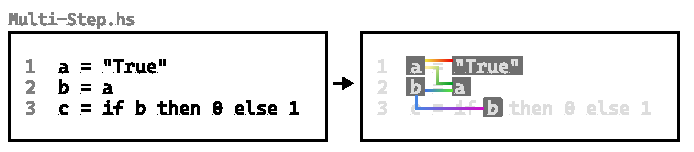
\includegraphics[width=\linewidth]{Multi-Step}
  \caption[This illustration depicts a multi-step type error in Haskell]{
    \label{fig:multi-step-example}
    This illustration depicts a multi-step type error in Haskell. In the program (left panel), the string literal \texttt{"True"} is assigned to the variable \texttt{a} on line 1, followed by the assignment of \texttt{a}'s value to variable \texttt{b} on line 2. Subsequently, on line 3, the program attempts to use \texttt{b} as a boolean condition in an \texttt{if} expression. The error analysis can be visualized as a "chain" of reasoning, represented by the continuous line (right panel), tracing the propagation of the type mismatch through the sequence of assignments and usage. }
\end{figure}

A \textbf{multi-witness type error} involves multiple pieces of evidence supporting the same potential type assignments. For instance, as shown in Figure \ref{fig:multi-witness-example}, multiple evidence (lines 3,4,5) support that \texttt{a} has the type \texttt{Int -> String}. On the other hand, a single piece of evidence (line 2) shows that \texttt{a} has the type \texttt{Int -> Char}.  Clarifying and juxtaposing this discrepancy in witnesses is key to supporting understanding this type of error.

\begin{figure}[htbp]
\centering  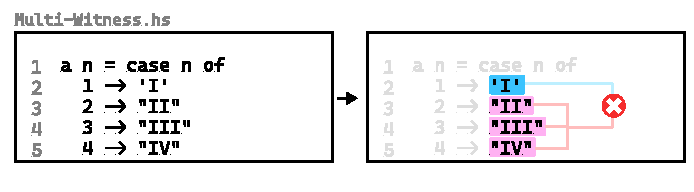
\includegraphics[width=\linewidth]{Multi-Witness}
  \caption[This illustration depicts a multi-witness type error in Haskell]{
    \label{fig:multi-witness-example}
    This figure presents the analysis of a multi-witness type error in Haskell. In the source code (Left), a type conflict arises from the \texttt{case} expression, which could be interpreted as \texttt{Char} based on the value in line 2, or as a \texttt{String} based on the values in lines 3, 4, and 5. The type conflict is graphically illustrated (Right) with \texttt{String} values marked in pink and the \texttt{Char} value in blue. The majority of \texttt{String} value witnesses suggest the lone \texttt{Char} literal \texttt{'I'} on line 2 might be a typographical error. This discrepancy underscores the significance of witness count in identifying the likely error source.}
\end{figure}

A \textbf{multi-party type error} involves several potential type assignments, each supported by distinct evidence.  Figure \ref{fig:multi-party-example} presents a typical multi-step type error: the expression \texttt{d} can not be assigned a type because 3 pieces of evidence on line 1 suggest 3 potential types for \texttt{d}. In practice, addressing such errors requires breaking them down into multiple type errors of simpler forms.


\begin{figure}[htbp]
\centering  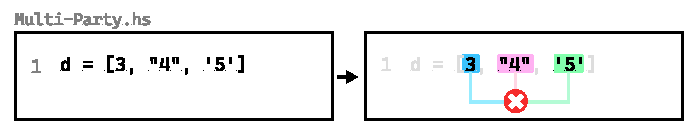
\includegraphics[width=\linewidth]{Multi-Party}
  \caption[This illustration depicts a multi-party type error in Haskell]{
    \label{fig:multi-party-example}
    This figure analyzes a multi-party type error in the source code (Left), where the list \texttt{d} could potentially be typed as \texttt{[Int]}, \texttt{[String]}, or \texttt{[Char]}. The disagreement is visually represented (Right) by three distinct colors, each corresponding to the cause of one of the possible types. This scenario differs from previous examples as resolving the type error requires adjustments at multiple locations within the code, not just a single change.
       }
\end{figure}

These classifications have led to the development of three distinct systems—\chameleon{}, Goanna, and GeckoGraph—each designed to tackle unique challenges within the domain of type error debugging.

\subsection{Explain Multi-Step Type Errors Through Chain-Of-Thought Visualization}


We contribute \textbf{\chameleon{}}, an interactive Haskell debugging tool that identifies all relevant error-contributing locations and illustrates the logical relationships between these locations. 


Our contribution in \chameleon{} benefits from the existing work on Chameleon \cite{Stuckey2003-pz, Wazny2006-ll}. Originally,  Chameleon was developed as a command-line tool. Its novel ideal of interactive debugging allows programmers to view different possible type error explanations and type assignments by issuing console commands. Besides, Chameleon successfully encoded the Haskell type system, with the addition of functional dependency, entirely in constraint handling rules \cite{Fruhwirth1998-jq}. \chameleon{} shares the theoretical foundation with the original Chameleon, providing a modern implementation with many advanced features. Notably, \chameleon{} provides a novel debugging interface to interactively explore the chain of reasoning in a multiple-step type error, allowing programmers to interactively develop a panorama view of the type error. In addition, \chameleon{} uses an adaptive interface design; programmers can switch between different granularity of information based on their personal preferences. 


We conducted a series of three user studies to investigate the effect of type error slicing and interactive type error exploration. We compared how programmers solve type errors with \chameleon{} and with traditional compiler tools. Our findings show a notable improvement in debugging speed when using type error-slicing, particularly for complex tasks. Additionally, we observed a significant enhancement in debugging speed when programmers actively use the interactive debugging features, suggesting that interactive exploration of type errors can positively impact the debugging process.

\subsection{Resolve multi-witness and multi-party errors with Minimal Correction Subsets}

We provide \textbf{Goanna}, a Haskell type error debugging tool. Goanna enhances type error debugging in Haskell by identifying all relevant error-contributing locations and presenting all possible causes and their respective resolutions. It ranks the potential causes of type errors based on their likelihood, helping programmers identify the root causes with minimal interactions with the tool.


To evaluate the effectiveness of the MCS-based type error debugging approach, we compiled a dataset of 86 Haskell programs from various online discussion platforms, covering a broad spectrum of type error themes. We tested the accuracy of Goanna in identifying and resolving type errors, comparing it to traditional compiler tools. Our research confirms that Goanna consistently outperforms other tools in pinpointing the correct cause of errors. Moreover, Goanna's heuristics effectively narrow down potential causes and consistently include the real cause among its top suggestions. Although Goanna operates moderately slower than standard tools, its processing time remains sufficiently quick to offer real-time feedback to developers. 

\subsection{Visualizing Polymorphic Types}

We contribute \textbf{GeckoGraph}, a graphic notation for Haskell types. GeckoGraph encodes the same information as type signatures but uses colors, shapes, and symbols to make certain structures easy to identify at a glance. GeckoGraph uses visual elements to improve the understanding of complex type concepts, such as type classes and qualified constraints. GeckoGraph offers clarity when reading complex type signatures and comparing multiple types.

We conducted a large-scale user study to assess the effectiveness of GeckoGraph in improving upon the traditional text-based approach to type signatures. The user study was designed as an interactive puzzle game with gamification elements to boost participation and engagement. A total of 721 programmers, ranging in experience levels, took part in the study. The findings indicated that while GeckoGraph did not enhance the speed or overall success rate of problem-solving significantly, it was notably beneficial in aiding beginners with more challenging tasks. Feedback gathered through a qualitative post-study survey was positively inclined, highlighting that GeckoGraph is intuitive, non-intrusive, and helpful.

% \section{Research Method}

% \subsection{Human-centered programming language studies}

% One important decision that shape a lot of my work is employing human-centered research methods with our novel programming language systems. The adopting of human-centered methods happens at every stage of the projects: prototyping, development and evaluation. Although the using of these methods are not new at all, but they certainly are not the most polular choices in programming language studies.

% The motive of such decision is that it is impossible to understand what are the good qualities of type errors without observing how human use type errors to gain understanding. 


% The downside of study programming language is iterative design is very hard. programming tasks involves complex inputs and outputs, and it is very hard to study an incomplete system without a fully working systems. For instance, if we are to study the effect of type errors, it is most effective to have a system that can recognize type-correct program from ill-typed one. It is hard to evaluate with a mock-up or wizard of oz style fake outputs to study users' interaction.  To address this limitations, we have a few ideas implemented in our research:

% A minimal but practical set of language 
% Design for human from start



\section{Thesis outline}

 This thesis is structured into two main parts. The initial chapters (Chapters \ref{chap:introduction}, \ref{chap:haskell-type-checking}) build a comprehensive foundation on type systems and programming languages, setting the stage for our research contribution in subsequent chapters. The latter chapters focus on distinct contributions that tackle various challenges in type error debugging.

\subsection{Chapter 1: Introduction}
Chapter 1 sets the stage by discussing the fundamental concepts of programming languages and type systems. It explores the trade-off between enhancing program safety and optimizing usability, a central dilemma in programming language research and software engineering practice. The chapter highlights common issues and technical challenges associated with type errors, establishing the motivation for this research. It also outlines the specific aim and contributions of the study, providing a roadmap for the thesis.

\subsection{Chapter 2: Haskell Type Checking}
This chapter delves into the fundamental concepts underlying type systems and programming languages. It outlines traditional methods employed in Haskell type checking, error slicing, and interactive debugging. Additionally, this chapter discusses tools and techniques used in constraint satisfiability analysis that are integral to later developments in the thesis. The categorization of type errors is revisited and redefined, building on the definitions introduced in this chapter.
    
\subsection{Chapter 3: \chameleon{} -- Interactive Type Error Visualization and Exploration}
Chapter 3 presents \chameleon{}, a system designed to enhance the debugging of type errors through interactive visualizations. It begins with a discussion on the typical pitfalls of existing error messages and outlines the motivation behind \chameleon{}. We then detail the system's design, features, and development process, including iterative prototyping. A series of empirical studies were conducted to assess \chameleon{}'s effectiveness compared to traditional compiler tools.
    
\subsection{Chapter 4: Goanna -- Finding All Type Errors Using Minimal Correction Subsets}
Chapter 4 introduces Goanna, a Haskell type error debugging tool that incorporates novel features such as suggesting fixes for type errors and cross-module debugging capabilities. It starts with highlighting the limitations of conventional compiler error messages and progresses to describe Goanna's capabilities in identifying all causes and ranking potential causes by their likelihood. The implementation tactics and heuristic methods used in Goanna are discussed, followed by an empirical evaluation of the system's accuracy, conciseness, and performance based on real-world Haskell code examples.
    
\subsection{Chapter 5: GeckoGraph — A Graphic Notation For Haskell Types}
Chapter 5 introduces our design of GeckoGraph. GechoGraph is a graphic notation for Haskell types. This chapter starts by underscoring the challenges of understanding and using polymorphic types. It then introduces GeckoGraph, how it addresses these challenges, and how to constructively transform text-based type signatures to GeckoGraph. We then showed our experiment on evaluating the effect of using GeckoGraph to help solve program tasks. Lastly, we discussed the strengths, limitations, and potential applications of GeckoGraph and type visualizations in general.   
    
\subsection{Chapter 6: Conclusion}
The final chapter reiterates the thesis's contributions. It discusses potential avenues for future tool development and research opportunities, forecasting the future landscape of programming language research. The chapter concludes with reflections on the importance of improving type error diagnositics, encouraging ongoing investigation and innovation.